\documentclass[a4paper]{article}

\usepackage{color}
\usepackage{url}
\usepackage[T2A]{fontenc} 
\usepackage[utf8]{inputenc} 
\usepackage{graphicx}
\usepackage{setspace} 

\usepackage[english,serbian]{babel}


\usepackage[unicode]{hyperref}
\hypersetup{colorlinks,citecolor=green,filecolor=green,linkcolor=blue,urlcolor=blue}

\newtheorem{primer}{Primer}[section]

\begin{document}

\title{Poređenje različitih vrsta prenosa podataka na mobilnom telefonu\\ \small{Seminarski rad u okviru kursa\\Tehničko i naučno pisanje\\ Matematički fakultet}}

\author{Andrija Soković\\ 
\small{andrijasokovic@gmail.com}
\and
Nenad Pešić\\
\small{pesicnenad28@gmail.com}
\and
Vojin Knežević\\
\small{knezevic.vojin9@gmail.com}
\and 
Vukašin Cupara\\
\small{vukasin.cupara2003@gmail.com} 
}
\date{14.~novembar 2022.}
\maketitle

\abstract{
U ovom radu obrađen je način funkcionisanja i sam koncept prenosa podataka na mobilnim telefonima. Obrađene su različite vrste tehnologija bežičnog prenosa i upoređene su njihove glavne karakteristike. Cilj teksta jeste da iznošenjem mogućnosti, prednosti i mana svake tehnologije, objasni svrha postojanja velikog broja različitih tehnologija za prenos podataka i polje primene svake od njih.}

\begin{spacing}{0.9}
    \tableofcontents
\end{spacing}

\newpage

\section{Uvod}
\label{sec:uvod}
\textbf{Razmena podataka} predstavlja proces pouzdanog slanja podataka izmedju dva ili većeg broja učesnika u komuniciranju. Ovim procesom moguće je slati mnogobrojne vrste podataka od kojih su najčešći: računarski fajlovi, digitalizovani signali slike, telemetrijski merni rezultati (npr. Podaci o merenjima temperature sa nekog senzora), centralne baze za nadgledanje itd.
U osnovnom obliku razmene podataka moguće je ostvariti komunikaciju između dva direktno povezana računara putem odgovarajućeg medijuma za prenos. Međutim, vrlo često, ovakav vid komunikacije nije dovoljan i pojavljuje se potreba za povezivanjem više računara. Tada je najpovoljnije povezati uređaj u neku već postojeću mrežu koja je organizovana po određenim standardima.\cite{racunarskeMreze} \\
Iako ne postoji opšta (zvanična) kategorizacija računarskih mreža, neformalno, mi računarske mreže možemo podeliti u dve grupe:
\begin{itemize}
\item Broadcast mreže (emisija svima)
\item Point-to-point (između 2 računara)
\end{itemize} 
Pored ove logičke podele računare fizički možemo povezivati različitim medijumima za prenos. Tu takođe možemo ostvariti neformalnu podelu na dve kategorije mreža u zavisnosti od vrste medijuma koji se koristi pri razmeni podataka:
\begin{itemize}
\item Žične računarske mreže (fizički medijum, npr. Bakarni kabl)
\item Bežične računarske mreže (medijum je etar, vazduh)
\end{itemize} 

\section{Bežične mreže}
Mobilni telefoni dizajnirani su na način koji predviđa upotrebu bežičnih mreža za međusobnu komunikaciju. Bežične mreže, prema svojoj topologiji možemo razvrstati u tri zasebne kategorije:
\begin{itemize}
\item Ad-hoc
\item Celularne (ćelijske)
\item Point-to-point
\end{itemize} 
    \subsection{Ad-Hoc}
Uspostavljanje komunikacije među uređajima vrši se direktno, bez unapred obezbeđene infrastrukture. Omogućava se veza „svako sa svakim“ bez pristupnih stanica. Poruka putuje kroz mrežu koristeći čvorove kroz koje prolazi, pri čemu svaki uređaj u mreži postaje i čvor. Pod terminom čvor, podrazumeva se svako mesto u mreži na kojem može doći do „grananja“, odnosno, promene smera paketa (poruke) koji se prosleđuje kroz mrežu. Ovakve mreže su pogodne za komunikaciju između manjih grupa korisnika na malom rastojanju i primenjuju se uglavnom tamo ge je neophodno brzo uspostaviti privremenu mrežu.\\
Na slici \ref{fig:adhoc} prikazan je dijagram Ad-Hoc mreže. Svaki uređaj priključen je na mrežu zasebno i putem mreže može da komunicira sa bilo kojim uređajem na mreži nezavisno (bez mrežne infrastrukture). 
\newpage

\begin{figure}[ht!]
\begin{center}
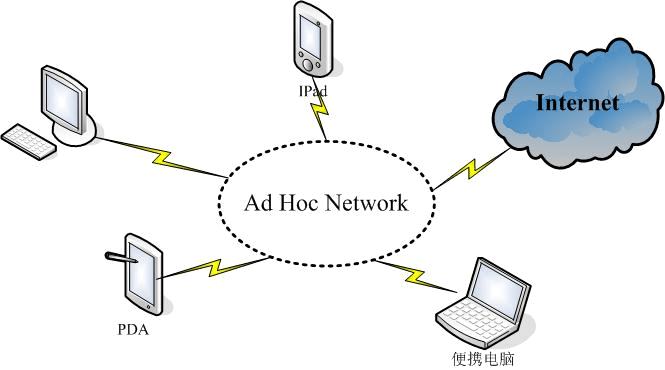
\includegraphics[scale=0.35]{AdHoc.png}
\end{center}
\caption{Ad-Hoc \cite{AdHoc}}
\label{fig:adhoc}
\end{figure}



    \subsection{Ćelijske mreže}
 Kod mreža sa ćelijskom topologijom uređaji ne mogu da komuniciraju direktno između sebe, već je neophodno da se sva komunikacija vrši preko unapred postavljenih pristupnih stanica. U ovakvim mrežama za komuniciranje je neophodno da postoji određena infrastruktura. Izraz ćelijske mreže odnosi se na to da se jedno celo geografsko područje deli na određeni broj manjih područja pokrivenosti pristupnih stanica, odnosno ćelija.

    \subsection{Point-to-point}
\textbf{Point to point} mreže omogućavaju komunikaciju tačno dva uređaja bez potrebe za dodatnom infrastrukturom. Ovakve mreže koriste se uglavnom za privremenu komunikaciju dva uređaja koja se međusobno nalaze na maloj udaljenosti.

\section{Bezbednost}	
\label{sec:Bezbednost}

Kao važna karakteristika svake računarske mreže ubraja se i bezbednost iste. Različite vrste mreža podlozne su različitim napadima i obezbeđene su različitim metodama zaštite.
Uopšteno posmatrajući postoje tri različite vrste napada na mrežu (bežičnu mrežu):

\begin{itemize}
    \item Napadnuta fizička sigurnost mreže
    \item Neautorizovani napadi i prisluškivanje
    \item Ugrožavanje bezbednosti unutar same mreže od strane autorizovanog korisnika
\end{itemize}


\section{Vrste bežičnih mreža koje koriste mobilni telefoni}
\label{vrste_mreza_na_telefonu}

Nakon uspostavljanja osnovnih podela i karakteristika bežičnih mreža uopšteno, treba posmatrati i različite standarde, odnosno različite tehnologije bežične komunikacije koje koriste mobilni telefoni. Ipak pre pominjanja samih tehnologija, neophodno je izvršiti još jednu kategorizaciju istih prema nameni i području koje iste pokrivaju:

\begin{itemize}
    \item WWAN (Wireless Wide Area Network)
    \item WLAN (Wireless Local Area Network)
    \item WPAN (Wireless Personal Area Network)
\end{itemize}
    \subsection{WWAN (Wireless Wide Area Network)}
WWAN je mreža koja pokriva veliko geografsko područje. Ona vrši komunikaciju rastavljanjem “poruke” (podatka koji želimo da pošaljemo) na veliki broj malih delova koji se nazivaju paketi. U WWAN spadaju mrežne tehnologije poput: \textbf{LTE}, \textbf{GSM}, \textbf{CDPD}. 
        \subsubsection{GSM}
GSM tehnologija je prva verzija razmene podataka koja se (u svojoj novijoj realizaciji) i dalje koristi pri povezivanju telefona na mobilnu mrežu. Ovo je druga generacija mobilnih mreža (tzv. 2G). Razvijena je početkom devedesetih godina prošlog veka.
GSM koristi ćelijsku topologiju mreže. Upotrebljava se više baznih stanica koje pokrivaju svoja geografska područja (do 35 kilometara dometa). Ovo je prva verzija mobilne mreže koja koristi digitalnu tehnologiju za komunikaciju.
Svaka bazna stanica ima frekvenciju na kojoj radi i oblast koju pokriva (ćeliju). Ćelije se šematski prikazuju kao pravilni šestougaonici, čime se omogućava da su sve susedne stanice na istoj udaljenosti. Pri ovoj podeli, svake dve susedne stanice moraju da koriste različite frekvencije kako ne bi smetale jedna drugoj. \\
Glavne usluge koje GSM pruža su:
\begin{itemize}
    \item Prenos govora
    \item Prenos podataka (9.6 Kb/s)
    \item Slanje SMS (Short Message Service) poruka
\end{itemize}
Mobilni uređaj, koji pristupa mreži,  sastoji se od samog mobilnog telefona (terminala) i memorijske kartice, takozvane SIM (Subscriber Identity Module) kartice. SIM kartica sadrži međunarodni broj za identifikaciju pretplatnika IMSI (International Mobile Subscriber Identity) kojim se pretplatnik najavljuje na sistem, zatim, tajni kod za verifikaciju i druge informacije.

Na slici \ref{fig:GSM} je prikazan uprošćen dijagram GSM mreže.

\begin{figure}[!ht]
\begin{center}
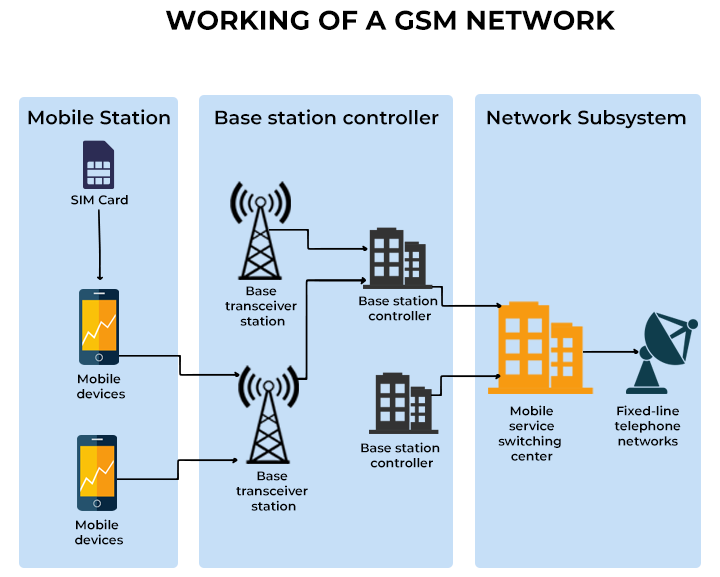
\includegraphics[scale=0.35]{GSM.png}
\end{center}
\caption{GSM mreža \cite{GSM}}
\label{fig:GSM}
\end{figure}
\newpage
        \subsubsection{LTE}
LTE tehnologija predstavlja naslednika GSM tehnologije (nekoliko generacija posle nje) i polja primena ove dve tehnologije se gotovo u celini poklapaju, s tim da LTE donosi mnogo benefita u odnosu na GSM.\\
Prilikom rada na LTE tehnologiji, istraživači su postavili nekoliko ciljeva i stavki koje LTE mora da ispunjava. Primarno je zahtevano smanjenje “cene po bitu” odnosno, radilo se na tome da za isti novac možemo preneti veću količinu podataka i samim tim dobiti ekonomičniju mrežu. Usko povezano sa tim bilo je i povećanje aspekta servisa koje ova tehnologija pruža. Sve je ovo naravno moralo da bude ispunjeno u skladu sa prvim zahtevom tako da LTE na kraju obezbeđuje “više servisa po nižoj ceni sa boljim korisničkim iskustvom”\\
Sa pogleda realizacije ove tehnologije, zahtevano je da LTE ispuni još nekoliko stavki. LTE je sa te strane dosta fleksibilnija sa upotrebom postojećih kao i sa uvođenjem novih opsega frekvencije za komunikaciju. Obezbeđena je jednostavnija arhitektura i umanjena je energetska potrošnja baznih stanica.\\
LTE korisnicima donosi brzine razmene podataka od 100 Mbps prilikom preuzimanja i od oko 50 Mbps prilikom slanja podataka. Smanjeno je vreme odziva prilikom komunikacije koja uključuje razmenu IP paketa (latencija je u većini slučajeva manja od 10ms).

    \subsection{WLAN (Wireless Local Area Network)}
U WLAN mreže spadaju sve one mreže koje za komunikaciju koriste radio talase. “Skelet” mreže čine pristupne stanice, na koje se povezuju bežični uređaji (npr. Mobilni telefoni), koje su “u pozadini” povezane kablovima. Ovakve mreže mogu imati promenljiv domet (mogu da pokrivaju samo jednu prostoriju a mogu i čitave kampuse). Na primer, u ovu kategoriju spada Wi-Fi tehnologija koja se danas uzima kao sinonim za bežične mreže.
        \subsubsection{Wi-Fi}
Wi-Fi predstavlja tehnologiju koja omogućava bežičnim uređajima (između ostalog i mobilnim telefonima) da se povežu međusobno na lokalnom nivou, a u velikoj većini slučajeva i da se povežu na globalnu mrežu, odnosno internet. Ruter se na internet povezuje infrastrukturom koju obezbeđuje internet provajder.(npr. Kablovsko povezivanje).\\
U suštini, putem pristupne stanice, bežični uređaj povezuje se na wireless ruter, odnosno uređaj koji će mu omogućiti pristup internetu. Pristupna stanica u suštini, služi kao posrednik između mobilnog uređaja i rutera, odnosno omogućava njihovo povezivanje bez fizičkog medijuma. Takođe uloga pristupne stanice jeste i da obezbedi korisne podatke o povezanim uređajima, obezbedi sigurnost mreže.\\
Za povezivanje uređaja putem Wi-Fi-a nije potrebna optička vidljivost između dva uređaja (odnosno mobilnog uređaja i pristupne stanice).\\
U zavisnosti od toga koji standard je implementiran Wi-Fi može da ima različite opsege brzine kao i dometa. Osnovni standard IEEE 802.11a podržava 54 Mbps. Noviji standardi dramatično su povećali protok podataka te je recimo po IEEE 802.11ac podržan protog do 3.5Gbps. Daljinska pokrivenost može dosegnuti od 70m (u zatvorenom prostoru) pa sve do 250m (na otvorenom proctoru), mada je uglavnom to domet od oko 30 metara. \cite{wireless} \\
Wi-Fi funkcioniše na dve glavne frekvencije: 2.4 GHz i 5GHz \\
        \subsubsection{Li-Fi}
Iako imenom podsećaju, Wi-Fi i Li-Fi su generalno dosta različite tehnologije.\\
Glavna razlika između njih jeste to što se Li-Fi oslanja na optičku vidljivost kao osnovni uslov komunikacije dva uređaja. Li-Fi prenosi podatke koristeći modulaciju jačine svetlosti. Osnovne dve komponente svakog Li-Fi Sistema jesu LED lampa (predajnik) kao i tzv. Li-Fi Dongle (prijemnik). \\
Korišćenjem Li-Fi tehnologije možemo ostvariti brzine do 1 gigabita po sekundi, dok vezu možemo ostvariti na udaljenostima od oko 10 metara.
Najčešće se primenjuje za prenos podataka među saobraćajnom signalizacijom, uličnom rasvetom i slično.\\

    \subsection{WPAN (Wireless Personal Area Network)}
Privatne Bežične Mreže (WPAN) služe za povezivanje uređaja koji se nalaze u međusobnoj blizini, takoreći u dosegu prosečne osobe (personal networks). Tipičan domet WPAN mreže je otprilike 10 metara. Često se koriste da umreže kompatibilne uređaje blizu neke centralne lokacije, kao recimo radnog stola. U ovu kategoriju spadaju tehnologije poput: Bluetooth, ZigBee, Infrared, NFC…

        \subsubsection{Bluetooth}
Bluetooth je tehnologija za bežičnu konekciju na malim distancama. Zamisao tehnologije jeste da posluži kao zamena za kablove u svakodnevnoj, ličnoj, upotrebi (npr. Za slušalice ili za miš).\\
Za ostvarivanje Bluetooth komunikacije nije potrebna optička vidljivost između dva uređaja. Funkcioniše u opsegu frekvencija od 2.4 do 2.485 GHz. Brzina prenosa podataka koja se ostvaruje prilikom Bluetooth veze je oko 700 Kb/s dok je gornja granica brzine, pri korišćenju osnovne verzije, 720 Kb/s. Ova granica brzine može biti podignuta sve do 3MB/s korišćenjem određenih tehnika kodiranja signala.
Domet koji ostvaruje Bluetooth veza je otprilike 10 metara. Vredi napomenuti da se brzina podataka smanjuje povećanjem udaljenosti dva uređaja, zbog smetnji koje se javljaju u prenosu signala.\\
Bluetooth je tehnologija koja koristi AD-Hoc tehniku povezivanja. Naime, formira se mreža od jednog uređaja koji je master uređaj i najviše 7 slave uređaja. Pored ovih primarnih 7, moguće je povezati još dosta uređaja koji nisu aktivani, tzv. “parkirani” uređaji, koji su na čekanju, ukoliko žele da uspostave konekciju, sve dok neki od aktivnih uređaja ne ode u stanje mirovanja i oslobodi mesto. Ovakva konfiguracija naziva se Piconet.\\
        \subsubsection{Infrared}
Infrared tehnologija bežičnog prenosa postoji već duži niz godina (duže od većine tehnologija pomenutih u ovom tekstu). Najčešće se sa njom možemo sresti u svakodnevnom životu, na primer gotovo svi daljinski upravljači  koriste baš ovu tehnologiju za komunikaciju (recimo sa televizorima). Danas se infrared može videti i u mobilnim telefonima, mada upotreba ove tehnologije nije toliko zastupljena u toj sferi.\\
Infrared koristi infra crvene zrake za razmenu podataka između uređaja. Ona omogućava veće brzine od Bluetooth konekcije, koje dosežu od 10 Mbps do 16 Mbps.
Kao što se može naslutiti, infrared zahteva optičku vidljivost između dva uređaja i komunikacija ne može da se proseže kroz fizičke prepreke. Može se koristiti „direktnim pogledom“ među uređajima, ali u nekim situacijama, signal se može prenositi i odbijanjem od neke prepreke (recimo zida). Usmeren način komunikacije omogućava pokriće distance od oko 3 metra, dok difuzioni način može da pokriva čitavu prostoriju sličnih dimenzija. \\
Ova tehnologija pruža bezbednu i jeftinu zamenu za kablove. Moguće ju je prilagoditi različitim okruženjima i funkcijama koje treba da ispuni.\\

        \subsubsection{NFC}
Near-field communication (NFC) predstavlja tehnologiju kratkog opsega koja koristi indukciju magnetnog polja za komunikaciju između uređaja kada se dodiruju ili se nalaze na distanci od nekoliko centimetara jedan od drugog. Ovakva komunikacija najčešće uključuje autentikaciju kreditnih kartica, prenos malih datoteka ili brzu inicijalizaciju neke druge tehnologije (sa većim mogućnostima komunikacije).\\
Gotovo svi moderni telefoni podržavaju NFC čipove i aplikacije, kao što su aplikacije za plaćanje bez potrebe za fizičkom kopijom kreditne kartice (Google Pay, Apple Pay). Originalno je bila zamišljena kao tehnologija koja će biti korišćena za razmenu datoteka na mobilnim telefonima ali zbog ograničavajućih faktora (poput brzine prenosa i veoma male udaljenosti koju pokriva), zamenjena je drugim tehnologijama.\\
NFC ograničava komunikaciju na veoma malu razdaljinu. Korisnik mora da dovede uređaj na distance od oko maksimalnih 10 centimetara. Međutim, veoma važna karakteristika NFC tehnologije jeste to da ne postoji potreba za napajanjem prilikom korišćenja osnovnih funkcija ove tehnologije (slušanje i odgovaranje na poruke). Ovo omogućava primenu ove tehnologije i na uređaje bez baterije, poput kreditnih kartica. \cite{NFC}\\

\subsection{Pregled glavnih karakteristika različitih vrsta mreža}
Svaku tehnologiju okarakterisali smo sa nekoliko stavki za koje smatramo da su najvažnije pri izboru tehnologije koja će biti korišćena pri komunikaciji. Na ovoj listi, između ostalog nalaze se: brzina prenosa podataka, pouzdanost, domet i spektar primena tehnologije.\\
Evo tabele sa svim vrenostima:\\
\begin{center}
\scalebox{0.9}{%
    \begin{tabular}{c|c|c|c} 
      \textbf{Vrsta bežičnog prenosa} & \textbf{Brzina prenosa (u Mbps)} & \textbf{Frekvencija (u MHz)} & \textbf{Domet (u metrima)} \\
      \hline
      GSM & 0.0096 & 890-960 & do 40000 \\
      LTE & 50/100 & 1900-2100 & do 8000 \\
      Bluetooth & 0.7-3 & 2400 & 10 \\
      Infrared & 10-16 & 3 x $10^{8}$ & 3 \\
      NFC & 0.4 & 13.56 & 0.1 \\
      Wi-Fi & do 3500 & 2400/5000 & 70 \\
      Li-Fi & do 1000 & 2 x $10^{8}$ & 10 \\
    \end{tabular}
}
  \end{center}

\section{Zaključak}
Pisanje našeg rada motivisano je nedostatkom informacija i neupućenošću generalne populacije o mogućnostima i primenama različitih tehnologija prenosa podataka. Veoma je očigledno da prenos podataka na modernim telefonima uopšte nije jedinstven ni jednoličan, stoga ne postoji ni jedna tehnologija koja bi mogla da zadovolji uopšteno sve potrebe, a da pritom ostane efikasna u svojoj komunikaciji.\\
Različite tehnologije, osim sa tehničke strane realizacije komunikacije, korisnicima omogućavaju potpuno različita korisnička iskustva i omogućavaju nesmetanu upotrebu mobilnih telefona u svakodnevnom životu.\\
Posmatrajući tabelu možemo lako zaključiti da je Wi-Fi bolji od drugih vrsta prenosa. Iako nema domet kao što imaju GSM i LTE, on ubedljivo ima najveću brzinu prenosa podataka i najvišu frekvenciju, i iz tih razloga se najviše koristi.
Primetno je da danas većina ljudi vrši neadekvatan izbor mrežne tehnologije za komunikaciju. Sumiranjem informacija na ovu temu, nadamo se da smo olakšali razumevanje i eventualni odabir potencijalnog načina umrežavanja. 




\addcontentsline{toc}{section}{Literatura}
\appendix

\iffalse
\bibliography{seminarski} 
\bibliographystyle{plain}
\fi

\begin{thebibliography}{}

\bibitem[1]{AdHoc} ResearchGate.net \emph{Structure of Wireless Ad Hoc Network}
\bibitem[2]{GSM} spiseworks.com \emph{What Is GSM (Global System for Mobile Communications)? Meaning, Working, Architecture, and Applications} 
\bibitem[3]{NFC} techtarget.com \emph{Near-field communication (NFC)}
\bibitem[4]{racunarskeMreze} bpa.edu.rs \emph{Rašunarske mreže}
\bibitem[5]{wireless} Computer Controls \emph{Wireless Networks}

\end{thebibliography}

\end{document}
